\documentclass[sigconf]{acmart}
% packages should be added as needed 
\usepackage{graphicx}

\usepackage{algorithm} % for algorithms
\usepackage{algpseudocode}

\usepackage{booktabs} % For formal tables

\usepackage{amsthm} % For claims
\theoremstyle{remark}

\pagestyle{plain} % removes running headers

\newcommand{\PicScale}{0.5}
\newcommand {\FlameStream} {FlameStream}
\begin{document}

\title {\FlameStream: Model and Runtime for Distributed Analytical Stream Processing}
% \titlenote{Produces the permission block, and   copyright information}
%\subtitle{Extended Abstract}
% \subtitlenote{The full version of the author's guide is available as   \texttt{acmart.pdf} document}

% \author {Igor E. Kuralenok \and Nikita Marshalkin \and Artem Trofimov \and Boris Novikov}

\author{Igor E. Kuralenok}
%\authornote{Dr.~Trovato insisted his name be first.}
%\orcid{1234-5678-9012}
\affiliation{%
  \institution{JetBrains Research}
%streetaddress{P.O. Box 1212}
  \city{St. Petersburg} 
%  \state{Ohio} 
%  \postcode{190000}
  \country{Russia}
}
\email{ikuralenok@gmail.com}

\author{Artem Trofimov}
\affiliation{%
  \institution{JetBrains Research}
  %streetaddress{P.O. Box 1212}
  \city{St. Petersburg} 
  \country{Russia}
}
\email{trofimov9artem@gmail.com}

\author{Nikita Marshalkin}
\affiliation{%
\institution{JetBrains Research}
  %streetaddress{P.O. Box 1212}
  \city{St. Petersburg} 
  \country{Russia}
}
\email{marnikitta@gmail.com}

\author{Boris Novikov}
\affiliation{%
\institution{JetBrains Research}
  %streetaddress{P.O. Box 1212}
  \city{St. Petersburg} 
  \country{Russia}
}
\email{borisnov@acm.org}


%\author{Artem Trofimov, Nikita Marshalkin, Boris Novikov}
%  \authornote{}
%\affiliation{%
%  \institution{St. Petersburg state University}
%  \streetaddress{Universitetskaya nab. 7/9}
%  \city{St. Petersburg} 
%  \postcode{199034}
% \country{Russia}
%}
%\email{trofimov9artem@gmail.com, marnikitta@gmail.com, borisnov@acm.org}


\begin{abstract}
Current generation of scalable distributed systems designed for analytical processing of large volumes of data have addressed drawbacks of previous generation. However, several issues still remain. Particularly, existing solutions suppose that the state of operations should be managed directly by user.

\FlameStream\ is a low-latency oriented distributed framework for executing analytical workflows. We offer a computational model that relieves user of explicit state handling and corresponding distributed environment that guarantees ``exactly once'' processing. The experiments show that prototype of our system is able to outperform alternative solutions.
\end {abstract}

\maketitle

\section {Introduction}
%%% fs-run-time-intro  - Introduction

\label {fs-intro-seciton}

A need to process huge amounts of data (e.g. Internet scale) was addressed by scalable distributed data processing systems such as  mapreduce. These systems are able to run data processing in a massively parallel mode on a clusters consisting of thousands of commodity computers. 

However, the initial models and frchitectures of this kind suffered from several drawbacks deeply analyzed in~\cite{Doulkeridis:2014:SLA:2628707.2628782,}. Many of these drawbacks were addressed in the next generation of scalable distributed data processing architectures, e.g. 
Asterix~\cite{Alsubaiee:2012:ASW:2331801.2331803}, 
Spark~\cite{Zaharia:2016:ASU:3013530.2934664,Franklin:2015:MSB:2684822.2685326}, 
and Flink~\cite{Carbone:2017:SMA:3137765.3137777}. 

The goal of the FlameStream (how should it be written? with a space or like here?) is to further improve performance and provide for better consistency of the output.  Specifically, the objectives are:

\begin {itemize}
\item ready on key: the output is delivered as soon as it is computed for every single key, rather than at the completion of  the whole workflow.
\item exactly once execution: each input item is processed exactly once even in case of partial system failures. 
\end {itemize}

A brief outline of the overall architecture and planned features: types, declarative workflow specification, ? ? ?

This paper introduces a run-time module of the  FlameStream. 
Add more details here.

The contributions of this paper are the following:

\begin {itemize}
\item definition of the computational model
\item implementation and proof of the concept.
\end {itemize}

The rest of the paper is structured as follows 
Describe sections here: model~\ref {fs-model-section}
implementation~\ref{fs-implementation-section}
experiments ~\ref{fs-experiments-section}
related work~\ref{fs-related-section}.


\endinput


\section {Computational model}
%%%% fs-run-time-data-flow  FlameStream data flow

\label {fs-model}

The key concept of \FlameStream\ model is a datastream. It is a sequence of discrete events described by data items, internally represented as 
$(Payload, Meta).$
The $payload$ is processed by a  user-defined code, while $Meta$ is handled with \FlameStream\ engine. In particular
the primary purpose of the meta-information is to impose the total order on data items. 
The  $Meta$ is assigned at the entry (called {\em  front}) and is discared at the {\em barrier} just before the exit. 

% \subsection{Computational flow}
The stream processing is specified by a logical execution graph. 
Each node of the graph represents a single operation on data items, and edges describe the routing of data items between operations.  
Our model allows cycles in the graph while such graphs are commonly assumed to be acyclic (DAGs) 
~\cite{Zaharia:2016:ASU:3013530.2934664, Carbone:2017:SMA:3137765.3137777}. 
The cycles are required for specification of certain computations (e.g MapReduce-based) with our spartan set of operation types (outlined below).
%Moreover, as we show further, there are cases when cycles are required, e.g., for MapReduce-based algorithms. 
Figure~\ref{logical-graph-figure} shows the example of logical execution graph.

% \subsection{Physical deployment and partitioning}
A distributed hardware environment is modelled as a set of {\em worker} processes. 
Each the workers executes logical execution graph and has an assigned range of hash values used for physical routing of data items to workers. 
%An integer interval (hash range) is assigned to every worker. Intervals are not intersected and cover the range of 32-bit signed integer.
%
Each operation input has a user-provided hash function called {\it balancing function}. This function is applied to the payload of data items and determines partitioning before each operation. After that, the data items are sent to the worker, which is responsible for the associated hash range. Therefore, load balancing explicitly depends on the user-defined balancing functions. 
%This allows the developer to determine optimal balancing which requires the knowledge of the payload distribution. The system optimizes the hash ranges assignment according to the processing statistics. 

\begin{figure}[ht]
  \centering
  \begin{minipage}[b]{.5\textwidth}
    \centering
    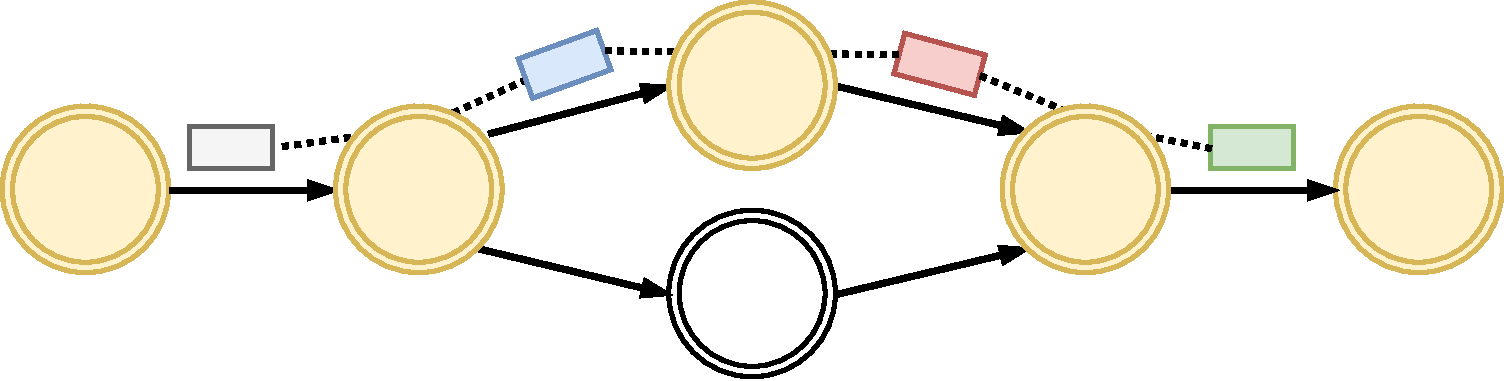
\includegraphics[width=0.9\linewidth]{pics/logical-graph}
    \caption{A logical execution  graph}
    \label{logical-graph-figure}
  \end{minipage}%
  \begin{minipage}[b]{.5\textwidth}
    \centering
    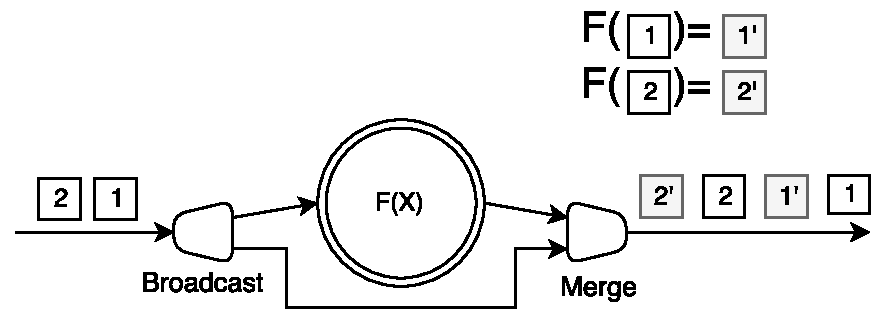
\includegraphics[width=\linewidth]{pics/ordering}
    \caption{The ordering model}
    \label{ordering}
  \end{minipage}
\end{figure}

% мм\subsection{Ordering model}

Data items are totally ordered according to lables assigned to events at the entry as a part of meta-information. All operations preserve this order. Any additional items produced by an operation are placed between the item being processed and the next item. The ordering labels are dropped when items are delivered from the barrier. 

% We assume that there is a total order on data items. 
% Ordering is preserved when an item is going through the operations. 
% More precisely, the order of output items is the same as the order of corresponding input items. 
% If more than one item is generated, they are inserted in output stream sequentially. 
% Moreover, the output follows corresponding input but precedes the next item. 
% Without diving into details, it should be noted that the order of items is maintained across different fronts.

The ordering is illustrated  in Figure~\ref{ordering}. Data item with payload $1'$ is the derivative of the item with payload $1$, according to operation $F$. The same is for items with payloads $2'$ and $2$. After merge operation, the order between $1$ and $2$ is preserved. Furthermore, $1'$ follows $1$, and $2'$ follows $2$.  

%  We assume that input items of the operations are strictly ordered.

%  \subsection{Operations}

The list of available operations includes:
\begin {description}
\item [Map] applies a user-defined function to the payload of an input item and returns a (possibly empty) sequence of data items with transformed payloads. 

\item [Broadcast] replicates an input item to the specified number of operations.

\item [ Merge] operation is initialized with the specified number of input nodes. It sends all incoming data to the output.

\item [ Grouping]  constructs a single item containing a set of consequtive items assigned to the same worker. The maximem nuber of items that can be grouped is specified as a parameter and is called window size. 
\end {description}

Grouping is the only operation that has a state.

%has a {\it window size} parameter. Grouping stores input items into distinct buckets by the value of the input balancing function applied to the payload. When the next item arrives at the grouping, it is appended to the corresponding bucket. Each time the grouping outputs window-sized {\it tuple item}, which consists of the most recent (in terms of the meta-information) items of this bucket. If the size of the bucket is less than the window, all items of the bucket are taken. 

The following example illustrates the semantics of the operation. The grouping accepts items with payload represented as natural numbers: 1,2,3, etc. The load balancing function returns 1 if the number is even and 0 otherwise. If the window is set to 3, the output is: \[(1), (2), (1|3), (2|4), (1|3|5), (2|4|6), (3|5|7), (4|6|8)...\]

The grouping operation has  two important properties: the output tuple is identified by its last element, the results among items with different values of a hash function are independent.

% \subsection{User-defined parameters}

% A user can set up the following parameters:

% \begin{enumerate}
%  \item{Computational flow}
%  \item{Balancing functions of the inputs}
%  \item{Map functions}
%  \item{Grouping windows}
%\end{enumerate}

%These parameters can produce more than one graph, which can yield equivalent results. Choosing among them is a performance optimization problem that relies on the system.
%It is important to mention that there are no parameters for state-management. 
%Therefore, business-logic is stateless. Nevertheless, the operations set is enough to implement any MapReduce transformation as shown in the next section.


\section {Optimistic collision management}
%%%% fs-run-mapreduce Optimistic collision management
\label {fs-collision}

As it was defined previously, only the grouping operation maintains a state and the state depends on the order of incoming items. Because of asynchrony and the possible existence of multiple paths between two nodes it is hard to deliver the right order.

In order to address this issue, we accept the fact that grouping can produce incorrect tuples. However, we guarantee that all correct tuples are eventually produced. The correctness of tuple means that this tuple would be generated if the order assumption was satisfied. 

To eventually produce all correct tuples, we use an approach called {\it replay}. If an item arrives the grouping operation, according to the meta-information order, nothing is replayed and only the most recent window is produced. However, if an item is out of order, it is inserted in the bucket at the correct location, and all tuples, which contain this element, are reproduced. Thereby, replay guarantees that eventually all correct tuples are generated. At the same time, for tuples, that has been produced but became invalid, {\it tombstones} are sent.

Tombstones are ordinal data items but with a special flag in its meta-information. This flag means that tuples with such meta-information are invalid, and they should not leave the system. Tombstones have the same payloads as invalid items in order to go through the same path in the computational pipeline.

The example of replay is shown in the figure~\ref{grouping-replaying}, The green item is out of order. The ouput consists of the new valid items, {\it (1, 2) and (2, 3)}, and the tombsone, {\it (1, 3)}.

\begin{figure}[htbp]
  \centering
  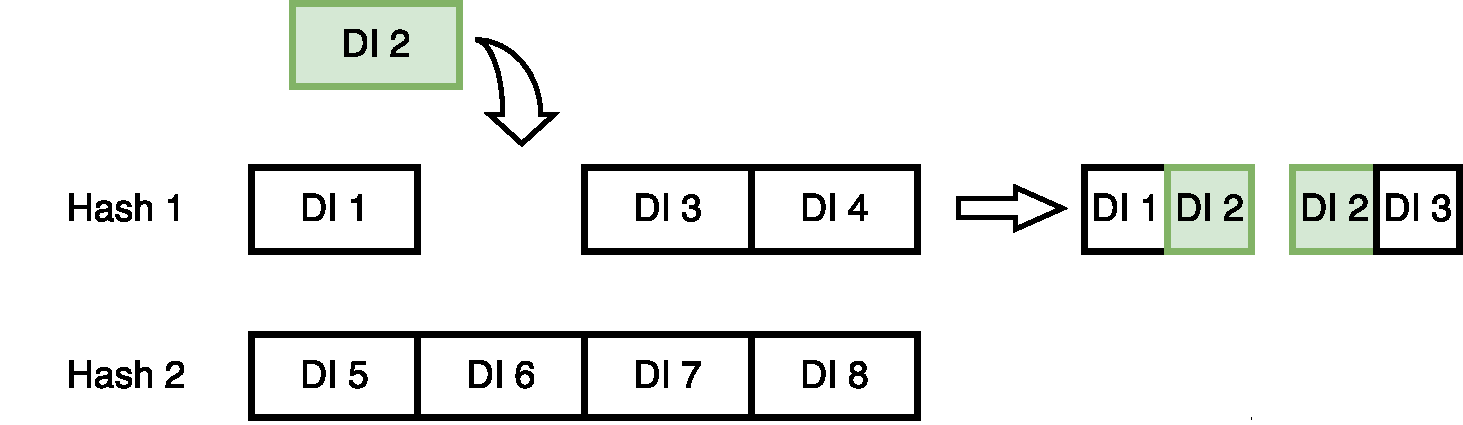
\includegraphics[width=0.48\textwidth]{pics/grouping-replaying}
  \caption{The replay in groupig with window = w. The new items are generated on insertion}
  \label {grouping-replaying}
\end{figure}

In the case of the right order of input items, there are no redundant items produced.

In order to filter out all invalid elements there is a need for {\it barrier} at the pipeline's sink, that filters invalid items when corresponding tombstones arrive. The barrier is partially flushed for some meta-information interval when there is a guarantee that there are no any out-of-order items and tombstones further up the stream for this range. The exact technique for providing such guarantee is defined further.

\subsubsection{Meta information}
The meta-information of data item is a tuple of a {\it global time}, a {\it trace}, {\it child ids} and a tombstone flag.

\[Meta := (GlobalTime, ChildIds[], Trace, IsTombstone)\]

Global time is assigned to data item once the item enters the system. It is a pair of milliseconds since the epoch start and the identifier of the front. The identifier is used to assign different global times to different items, even in case of wall-clock collisions. 

\[GlobalTime := (FrontTs, FrontId)\]

Global times are compared by front timestamp if they coincide - by front id. It is important to notice, that we are not relying on any clock synchronization between nodes, but we require a strict monotonicity within the single front. The only implication of the clock skew is the system degradation in terms of latency: 1ms of the nodes clock difference appends 1ms to minimal latency.

Each map operation can produce multiple items from one. This items are ordered between each other. To differentiate them the ordinal number, {\it child id}, is stored in the meta information. The {\it ChildIds } is an array of child ids, that corresponds to the all visited map operations.

The global time and child ids are enougth to uniquly identify data item within stream, if all processing is done without replays. If there are any replays happened during processing, multiple items with the same global time and child ids exists in the stream. There are multiple tombstones with the same global time and child ids can exist as well. They can take different paths in computational flow and travel within them with different speeds. 

Despite this fact, an invalid element and the tombstone for it are taking the same path, because they have the same payload and the balancing functions are determenistic. Moreover, the tombstome visits operations strictly after corresponding item, as links between operation are considered to be FIFO. To match tombstone with proper item there is {\it Trace} value stored in the meta-information.

Trace encodes the path item have traversed. Each phsical copy of each operation is assigned with unique random 64-bit identifier. The trace is a xor of the all operations' ids visited by item so far.

\[Trace := \bigoplus_{op \in \text{visited}} Id(op)\]

Metas are compared lexicographically. That is to say, firstly global times are compared, then child ids, then traces. Notice, this order is in line with the \FlameStream's ordering model.

The figure~\ref{logical-graph-ops-figure} shows the topology of each operation and how it affects the trace of local times.

\begin{figure}[htbp]
  \centering
  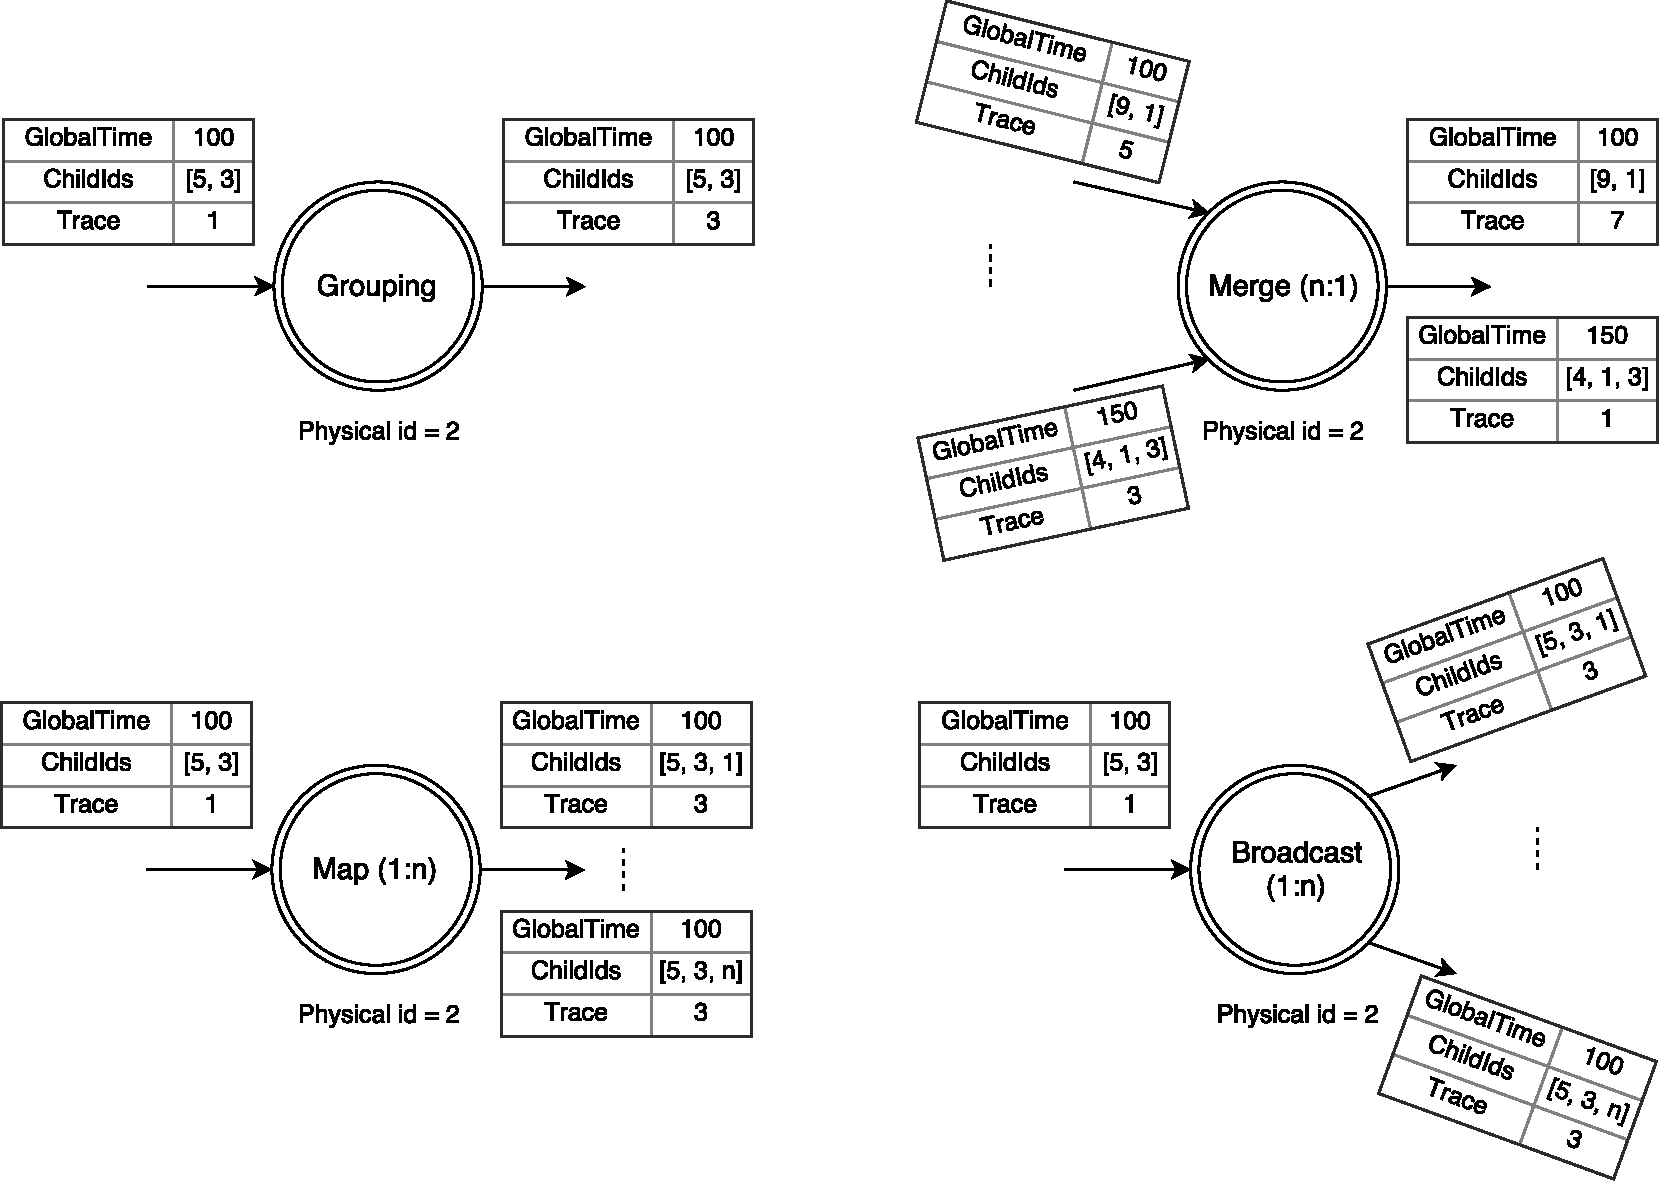
\includegraphics[scale=0.5]{pics/operations}
  \caption{Meta-information handling}
  \label {logical-graph-ops-figure}
\end{figure}

The structure of meta provides for tracking different relations between data items:

\begin{itemize}
  \item Items with same global time and common prefixes are produced from the same item
  \item Item with lower meta is generated earlier, at front or in the stream
  \item If there are two items with the same global time and child ids, only one of them is the right one
\end{itemize}

\label{mininal-time}
\subsection{Minimal time within stream}

To release the item from the barrier we need to ensure that there are no in-flight invalidators. 

\newtheorem{minimal-time-claim}{Lemma}

\begin{minimal-time-claim}
  If data item {\it D} has global time {\it GT} greater than the global time of the in-flight elements, then all tombstones for that item had already arrived at the barrier.
\end{minimal-time-claim}

\begin{proof}
  {\it RETHINK}
  Let {\it E} is in-flight element that invalidates {\it D}. According to the definition of invalidation order, {\it E} and {\it D} has the same global time {\it GT}, but the tombstone flag. We assumed that there are no in-flight element with the global time equal to {\it GT}. Contradiction.

  This implies that if the stream does not contain items with the global time less than or equal to {\it GT}, then all items which invalidate {\it D} had already arrived at the barrier. 
\end{proof}

Therefore, to output an item from the barrier, we should ensure that there are no items in the stream with the global time less than or equal to the global time of this item.

To track the global time of in-flight items we adopt an idea of {\it acker task} borrowed from Apache Storm~\cite{apache:storm}. Acker tracks data items using a checksum hash. When the item is sent or received by an operation, its global time and checksum are sent to the acker. This message is called {\it ack}. Acker groups acks by a global time into the structure called {\it ack table}. Once acker receives an ack message with global time {\it GT} and {\it XOR} it updates {\it GT} entry in the table by xoring {\it XOR} with the current value. When an item is sent and later received by the next operation, xoring corresponding {\it XOR}s would yield zero.

Acks are overlapped to nullify table's entry only when an item arrives at the barrier. That is, ack for receive is sent only after both processing and the ack sending for the transformed item, as illustrated in the figure~\ref{acker}. Different shapes of items mean different payloads. The ack for the sending of the triangular element is sent before the rectangular one. We expect the channel between the acker and each operation to be FIFO, so ack for the triangular item would be xored before the rectangular. So the two equal values are separated by distinct one. 

This technique guarantees that the {\it XOR} for some global time is equal to zero only if there are no in-flight elements with such global time.

\begin{figure}[htbp]
  \centering
  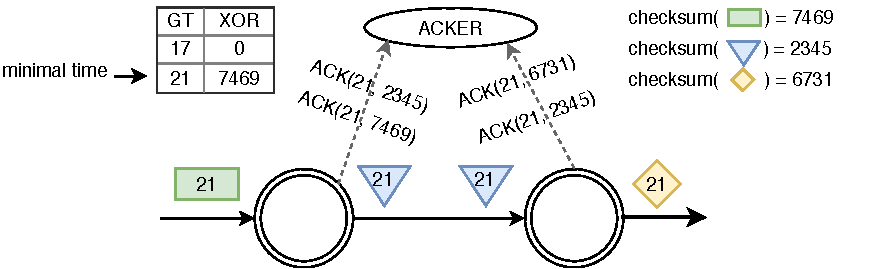
\includegraphics[scale=0.5]{pics/acker}
  \caption{Acker}
  \label {acker}
\end{figure}

The minimal time within a stream is the minimal global time with non-zero {\it XOR}. On minimal time changes, acker broadcasts new minimal time to the barrier and operations. Therefore, the barrier can release elements with global time {\it GT} once it received notification from acker that the minimal time within the stream is greater than {\it GT}.

To ensure that no fronts are able to generate item with the certain timestamp, each front periodically sends to acker special message called {\it report}, which promises that front will not generate items with a timestamp lower than the reported. The value in the ack table can become a zero only after the corresponding report arrives.

The proposed mechanism could be isolated by hash range. This change allows us making invalidation and releasing from barrier independent also known as early key availability.


\section {Implementation}
%%% fs-run-time-impl Implementation
\label{fs-impl}

\FlameStream\ is implemented in Java, using Akka framework for messaging. There are several main components within the implementation:
\begin{description}
  \item[Data producers and data consumers] are deployed separately and play the role of data source and data sink correspondingly.

  \item[Graph] is a component that is deployed on each node and executes a computational pipeline defined by a logical graph. Operations within the same node communicate with each other via direct function calls for performance optimization.

  \item[Barrier] filters out invalid data items. Besides, it delivers output items to data consumers.

  \item[Acker] tracks data items within the stream. Its functionality is detailed further.

  \item[Apache ZooKeeper] is used for cluster management. The usage of ZooKeeper mitigates the need for the dedicated master node.

  \item[Persistent storage] is needed for recovery in case of failures
\end{description}

The overall scheme of the system components is shown in Figure~\ref{system-architecture}.

\begin{figure}[ht]
  \centering
  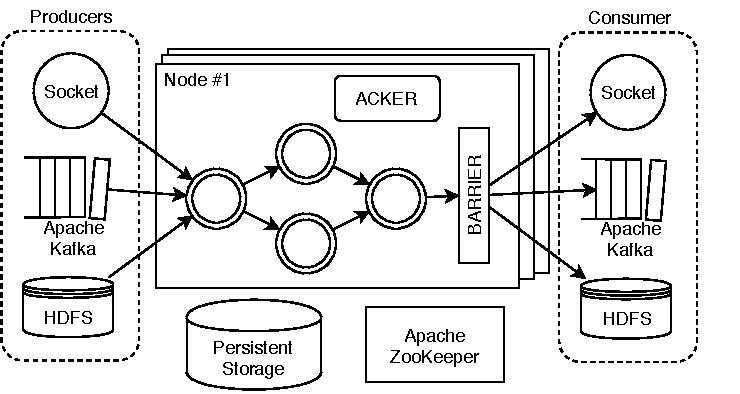
\includegraphics[width=0.70\textwidth]{pics/arch}
  \caption{The overall scheme of the system components}
  \label {system-architecture}
\end{figure}

\subsection{Ordering model}
The meta-information of data item is implemented as a tuple of a {\it global time}, a {\it trace}, {\it child ids} and a {\it tombstone flag}.

\[Meta := (GlobalTime, ChildIds[\:], Trace, IsTombstone)\]

Global time is assigned to data item once the item enters the system. It is a pair of logical time and the identifier of the front. The identifier is used to resolve time collisions within different fronts. It is important to notice that we do not rely on any clock synchronization between nodes. The only implication of the clock skew is the system degradation regarding latency: 1 ms of the fronts clock difference appends 1 ms to minimal latency.

Each map operation can produce multiple items from one.  An ordinal number, child id, is stored in the meta information to differentiate them. {\it ChildIds} is an array of child ids, that corresponds to all visited map operations.

The global time and child ids are enough to identify data item within a stream if all processing is done in-order. In this case, if we compare global time and child ids lexicographicaly the meta has the desired properties that were defined in section~\ref{model-section}. 

In order to filter out all invalid data at the barrier, there is a need to match tombstones with corresponding invalid items. However, if any grouping repairs happened during processing, multiple items with the same global time and child ids exist in the stream. To differentiate them without direct payload comparison, there is a {\it Trace} value stored in the meta-information. The trace is a xor of all physical operations' ids (random 64-bit identifier) visited by item so far. Invalid item and the corresponding tombstone go along the same path, because they have the same payload and the balancing functions are deterministic. Therefore, item and the corresponding tombstone can be revealed via trace matching. 

\label{mininal-time}

\subsection{Minimal time within stream}

To release an item from the barrier we need to ensure that there are no in-flight tombstones for that item, i.e., tombstones which have been already generated, but have not arrived at the barrier yet.

\newtheorem{minimal-time-claim}{Lemma}

\begin{minimal-time-claim}
For any data item $D$ let $\mathcal{G} (D)$ be its global time. 
  If data item $D$ has global time $\mathcal{G} (D) < \mathcal{G} (F)$ for each in-flight element $F$, 
  then all tombstones for that item had already arrived at the barrier.
\end{minimal-time-claim}

\begin{proof}
  Let $D_{tomb}$ be a tombstone for {\it D}. 
  According to the definition of the tombstone item, $\mathcal{G} (D_{tomb}) = \mathcal{G} (D)$, hence $D_{tomb}$ is not in-flight.
  
  New tombstones for $D$ cannot be generated because items with global time greater than $\mathcal{G} (D)$ cannot trigger repair that affects $D$,
  This implies that if the stream does not contain items $D\prime$ such that $\mathcal{G} (D\prime) \le \mathcal{G} (D)$, then all tombstones for $D$ had already arrived at the barrier. $\square$
\end{proof}

Therefore, to output an item from the barrier, we should ensure that there are no items in the stream with the global time less than or equal to the global time of this item.

To track the global time of in-flight items we adopt an idea of {\it acker task} inspired by Apache Storm~\cite{apache:storm}. Acker tracks data items using a checksum hash, called {\it XOR}. When the item is sent or received by an operation, its global time and checksum are sent to the acker. This message is called {\it ack}.
 Acker groups acks by a global time and xors received checksum hashes. 
When an item is sent and later received by the next operation, xoring corresponding {\it XOR}s would yield 0.

Acks are overlapped to nullify {\it XOR} only when an item arrives at the barrier. That is, ack for receive is sent only after both processing and the ack sending for the transformed item are done, as illustrated in Figure~\ref{acker}. This technique guarantees that the {\it XOR} for some global time is equal to zero only if there are no in-flight elements with such global time.

\begin{figure}[ht]
  \centering
  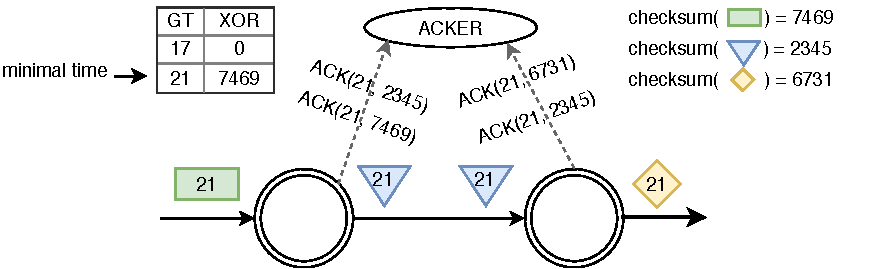
\includegraphics[width=0.8\textwidth]{pics/acker}
  \caption{The example of tracking minimal time using acker}
  \label {acker}
\end{figure}

The minimal time within a stream is the minimal global time with non-zero {\it XOR}. On minimal time changes, acker broadcasts the {\it new minimal time notification}. 
Therefore, the barrier can release elements with global time $\mathcal{G} (D)$ 
once it received notification with time greater than $\mathcal{G} (D)$.

To ensure that no fronts can generate item with the specific timestamp, each front periodically sends to acker a special message called {\it heartbeat} indicating that front will not issue items with a timestamp lower than the reported. The value in the ack table can become zero only after the corresponding heartbeat arrives.


\section {Experiments}
%%%% fs-run-time-experiments   Experiments

\label{fs-experiments-section}

\subsection{Setup}
We evaluated the series of experiments in order to estimate the performance of our system's prototype. As a stream processing task, we apply the computation of inverted index for Wikipedia documents. The computation of inverted index is implemented in terms of MapReduce transformations. We start with page mapping into the pairs {\it (word; word positions within the page)}. After that, word positions are reduced by word into the single structure. We assume the output of the stream to be change records of the inverted index structure, i.e. each input page triggers the output of the corresponding updates. 

Pairs {\it (word; word positions within the page)} must be ordered by page id and version before the update of inverted index state. Otherwise, it is possible to obtain the inconsistent index, if there are multiple versions of the same document.  
In the real-world, such scenario can be found in freshness-aware systems e.g. news processing engines. By the notion of {\it latency} we assume the time between two events: 
\begin{enumerate}
    \item Input page is taken into the stream
    \item All the change records for the page leave the stream
\end{enumerate}

In \FlameStream\ this algorithm is implemented as the typical conversion of MapReduce transformation, which is shown in section~\ref{fs-drifting}. Inverted index structure plays the role of an accumulator, and the accumulator map produces the most recent changes of this structure if any.

Our experiments were performed on the cluster of Amazon EC2 micro instances with 1GB RAM and 1 core CPU. We used 10000 Wikipedia articles as a dataset. 

\subsection{Overhead and scalability}

We take the ratio of arrived at the barrier items count to the number of the valid items among them as a key metric for the estimation of the overhead of our prototype. This value clearly represents the extra cost of our approach.

The relation between the number of workers, the delay between input documents and the proposed ratio is shown in Figure~\ref{overhead}. As expected, the peak of the ratio is achieved when the document per second rate is high, and the number of the nodes is low. This behavior can be explained by the fact that a few workers cannot effectively deal with such intensive load. Nevertheless, the proportion of invalid items reduces with the increase of workers number. Under non-extreme load, the total overhead of the optimistic approach is under 10\% for all considered number of workers. These results confirm that the ratio does not increase with the growth of the number of nodes.

\begin{figure}[htbp]
  \centering
  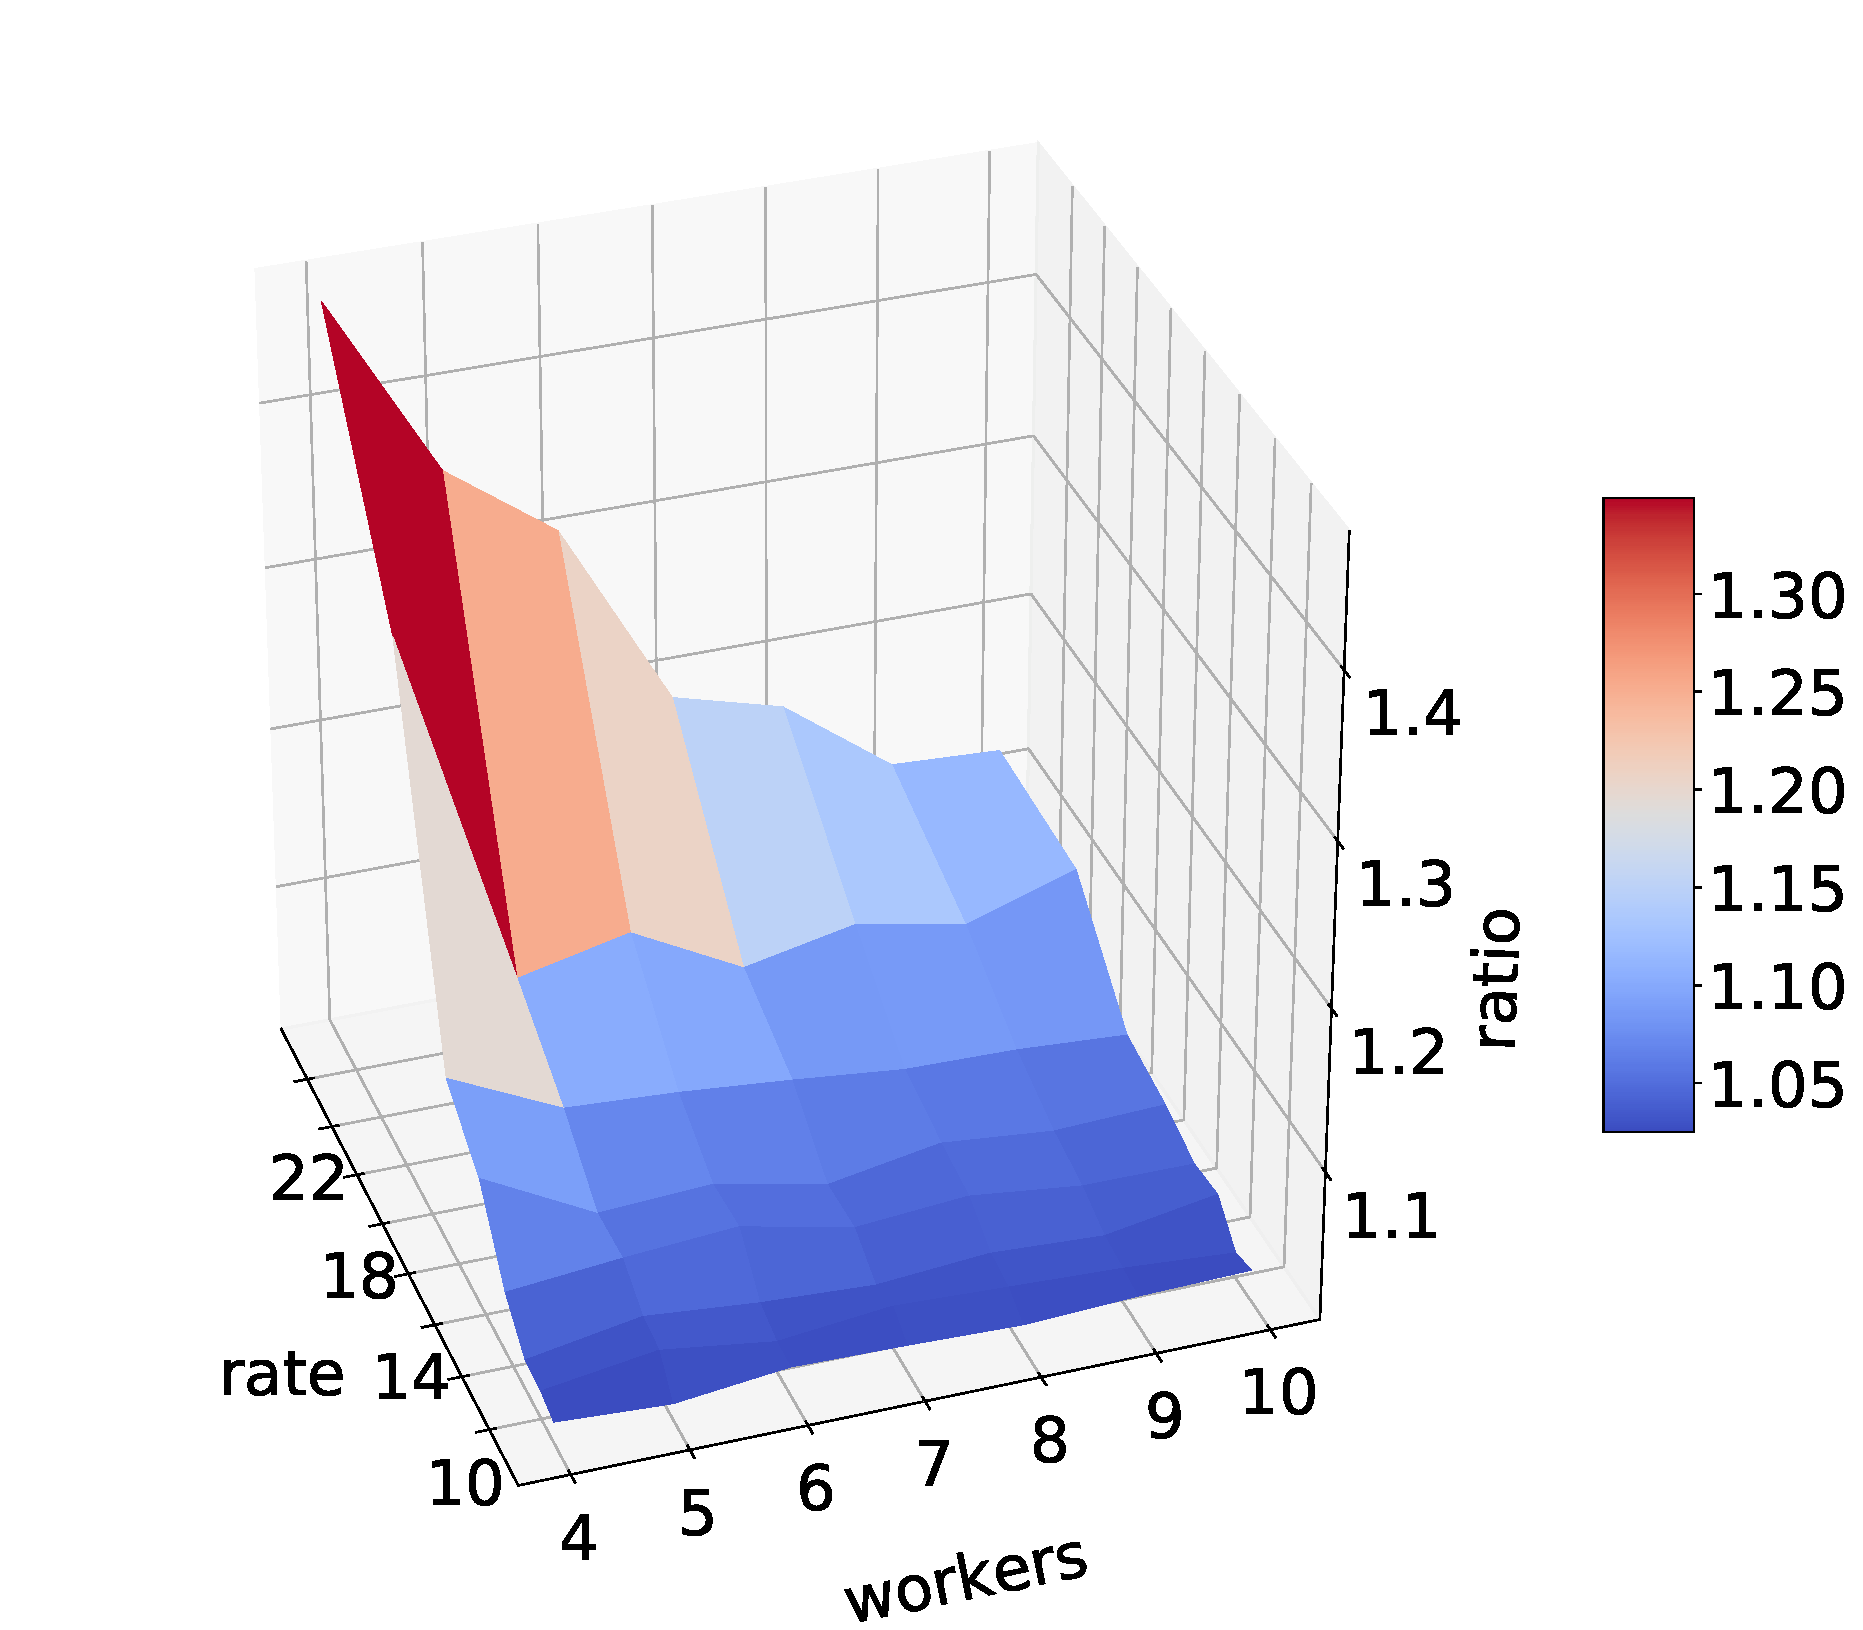
\includegraphics[width=0.5\textwidth]{pics/overhead}
  \caption{The relation between the number of workers, the delay between input documents and the replay ratio}
  \label {overhead}
\end{figure}

The latencies of \FlameStream\ across multiple workers for the fixed document rate of 70 ms are shown in Figure~\ref{fs-index-quantiles}. These figure demonstrate that latency is not significantly increased with the growth of the number of workers. 

Therefore, the most important conclusions of these experiments are: the proposed method is scalable, the overhead could be optimized by system setup.

\begin{figure}[htbp]
  \centering
  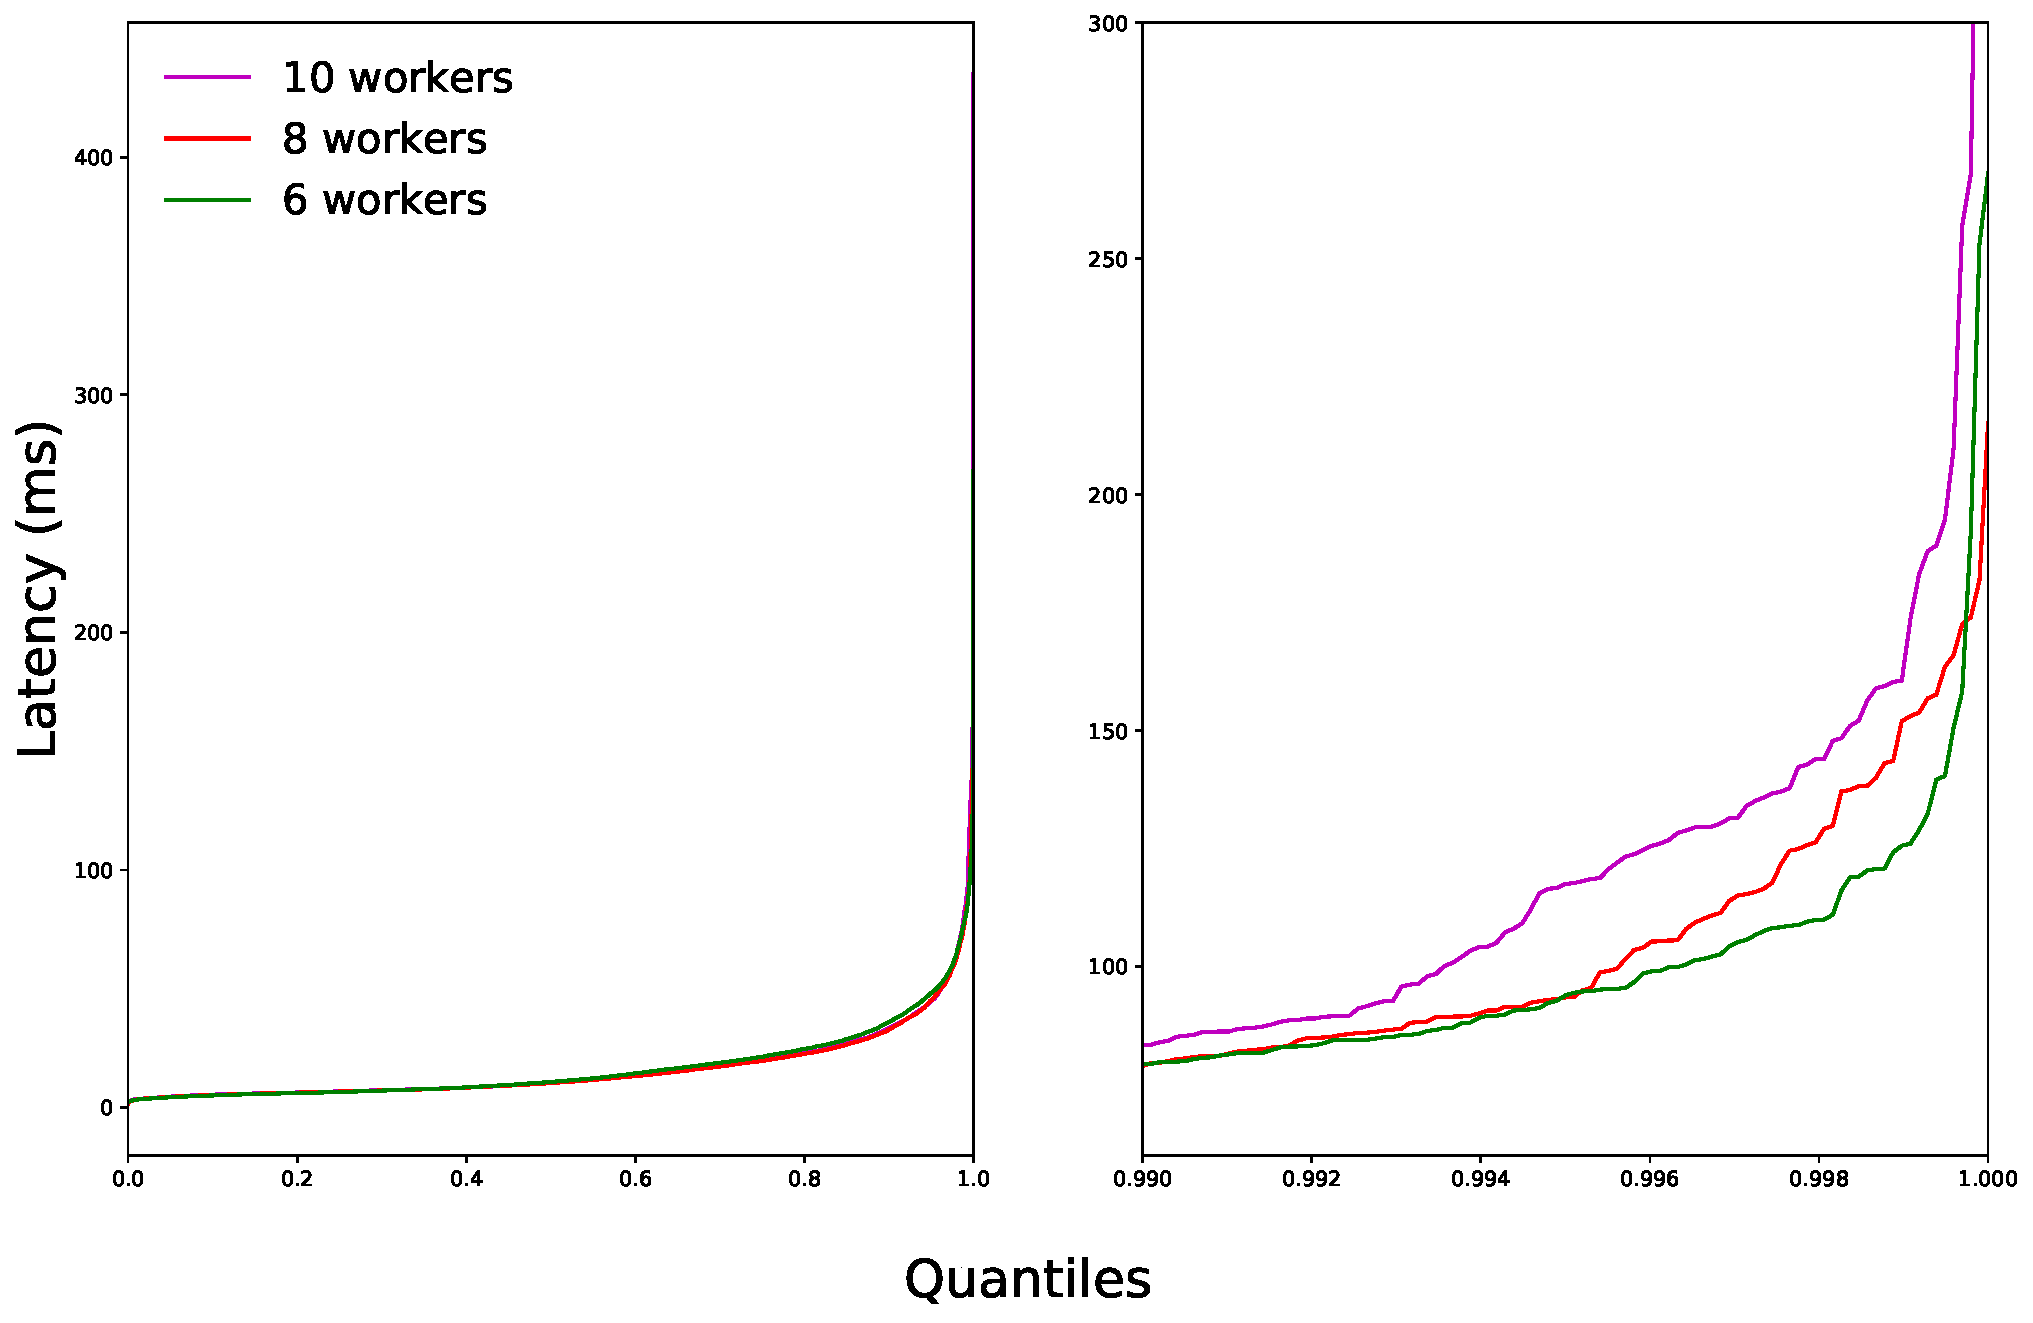
\includegraphics[width=0.48\textwidth]{pics/fs-index-quantiles}
  \caption{FlameStream latency distribution. Left - the whole distribution, right - tail latencies}
  \label {fs-index-quantiles}
\end{figure}

\subsection{Comparison against Apache Flink}

One of the most important goals of the experiments is the performance comparison with an industrial solution in terms of latency. Apache Flink is chosen for evaluation because it is state-of-the-art stream processing system that provides similar functionality and achieves low latency in the real-world scenarios~\cite{S7530084}. 

For Apache Flink, the algorithm for inverted index computation is adopted by the usage of {\it FlatMapFunction} for map step and stateful {\it RichMapFunction} for reduce step and for producing the change records. Order enforcing before reduce is implemented using custom {\it ProcessFunction} that buffers all input until corresponding low watermark is received. Watermarks are sent after each document. The network buffer timeout is set to 0 to minimize latency.

In this paper we compare $50^{th}$, $75^{th}$, $95^{th}$, and $99^{th}$ percentile of distributions, which clearly represent the performance from the perspective of the users' experience. Many papers report on averages, so these are included where it makes sense for comparison purposes. 

The comparison in latencies between \FlameStream\ and Flink within 10 nodes and distinct document rates is shown in Figure~\ref{fs-index-quantiles}. These results indicate that \FlameStream\ provides greater latency in the case of high load (25 rps). This fact corresponds with Figure~\ref{overhead}, which demonstrates that the overhead under such load is quite high. However, \FlameStream\ delivers better latency under less extreme loads. Firstly, the reason for such behavior can be the fact that Flink starts to update index only after the buffer before reduce stage is flushed. In contrast, \FlameStream\ flushes its barrier right before data is sent to a user, according to its optimistic nature. Secondly, low watermarks go along the stream and can be delayed by long-running operations, while acker processes ack messages independently. It is confirmed by Figure~\ref{buffer-vs-barrier}, which shows the comparison between waiting time in Flink's buffer and \FlameStream's barrier. 

\begin{figure}[htbp]
  \centering
  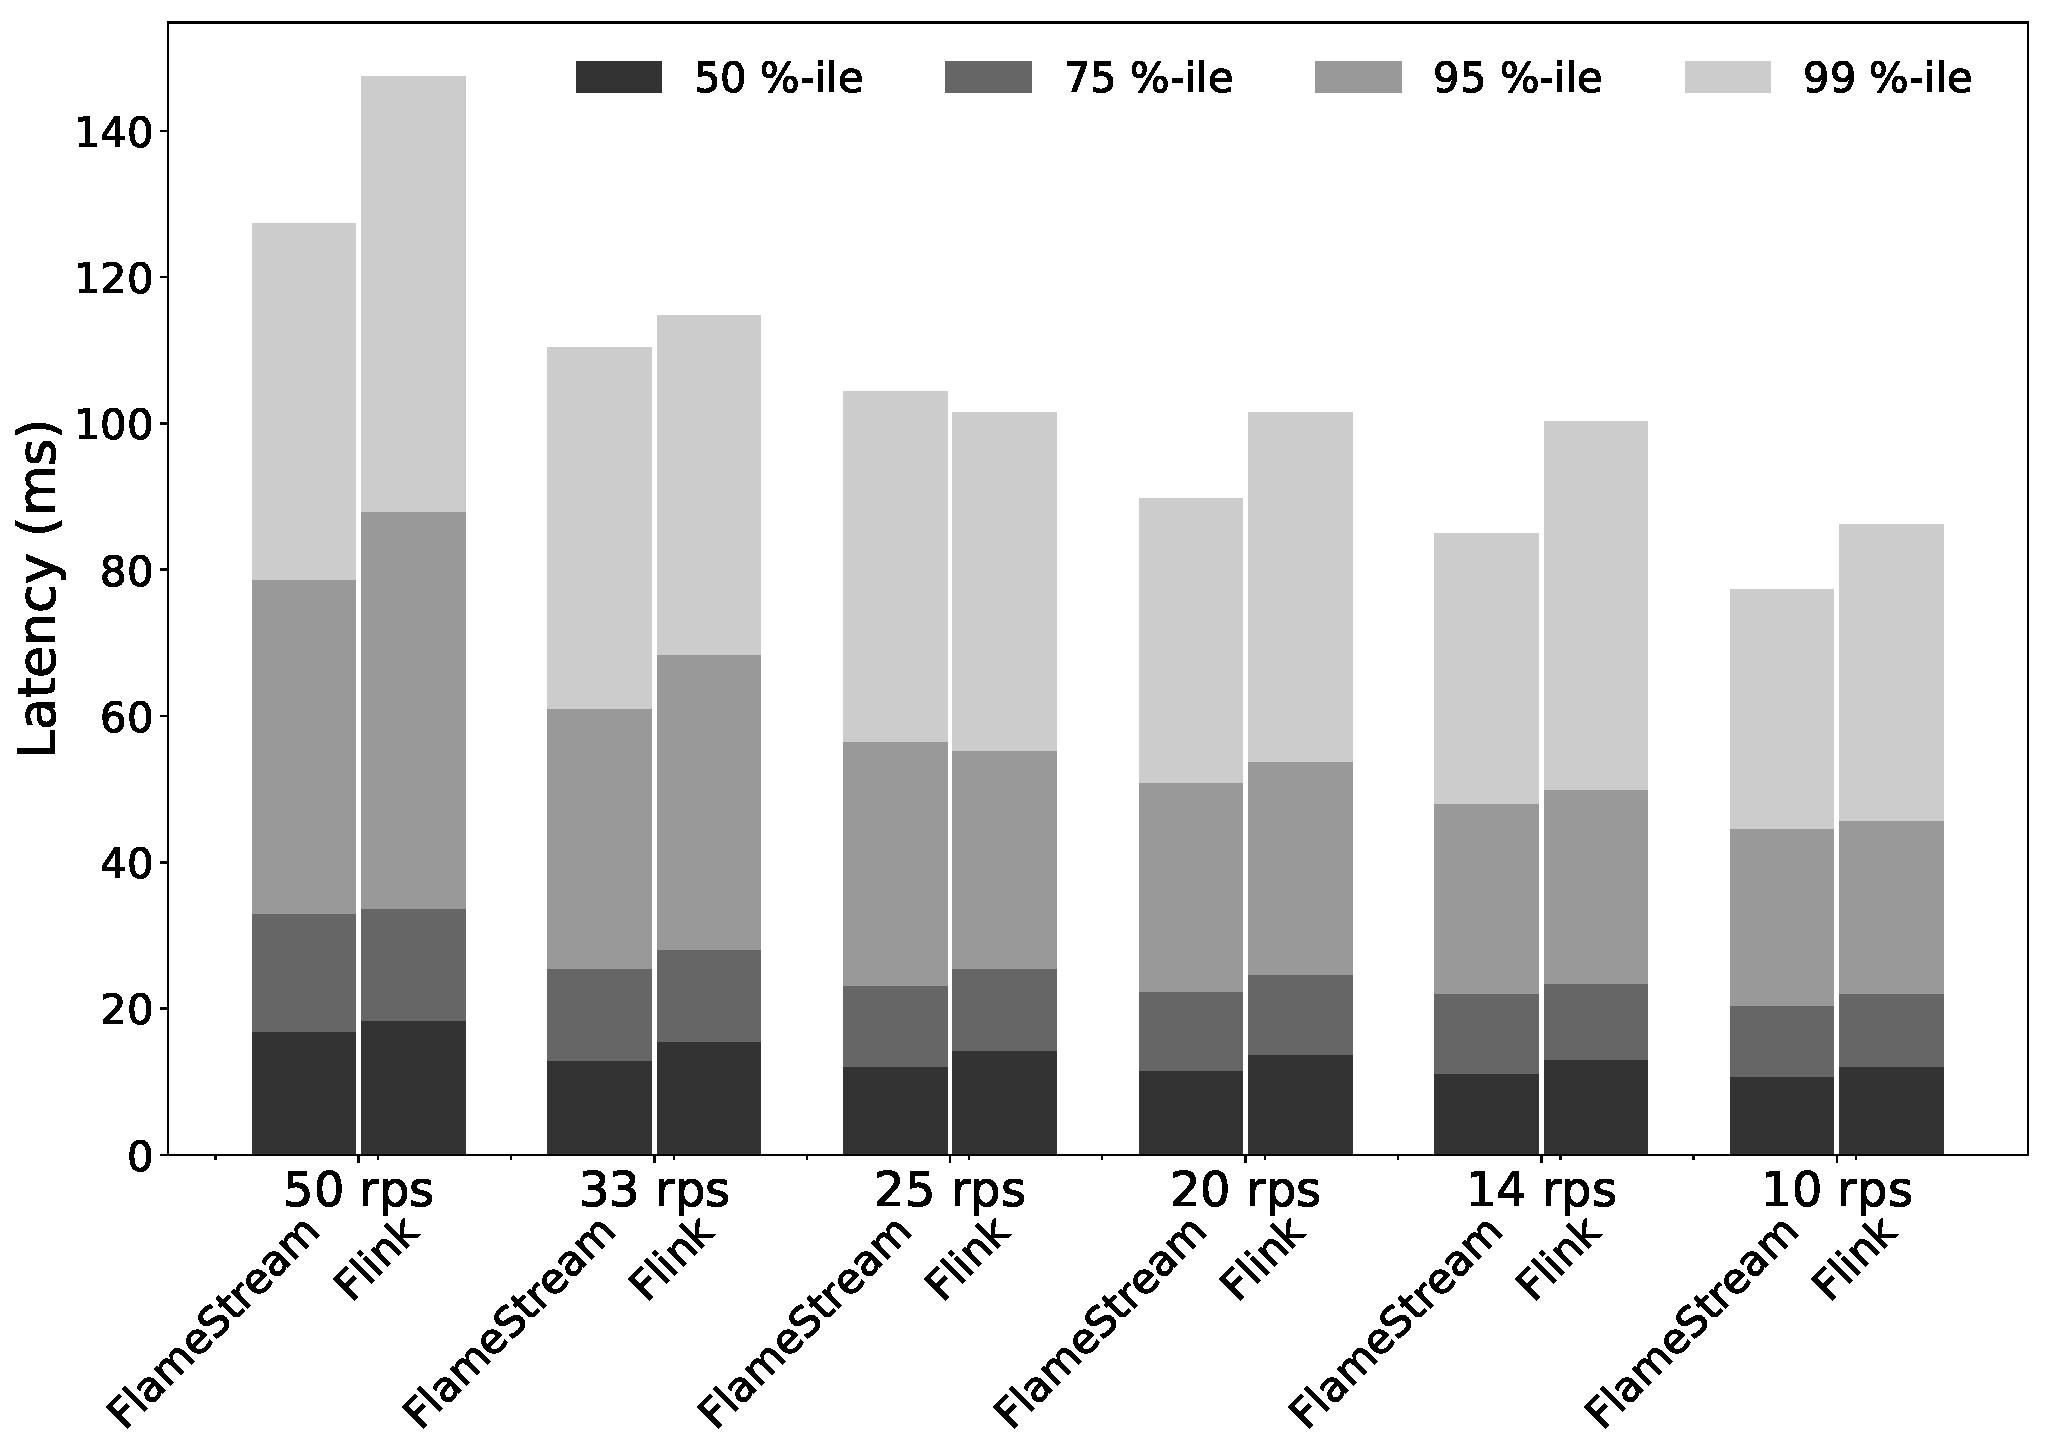
\includegraphics[width=0.5\textwidth]{pics/comp-index-quantiles}
  \caption{Latency comparison}
  \label {fs-index-quantiles}
\end{figure}

\begin{figure}[htbp]
  \centering
  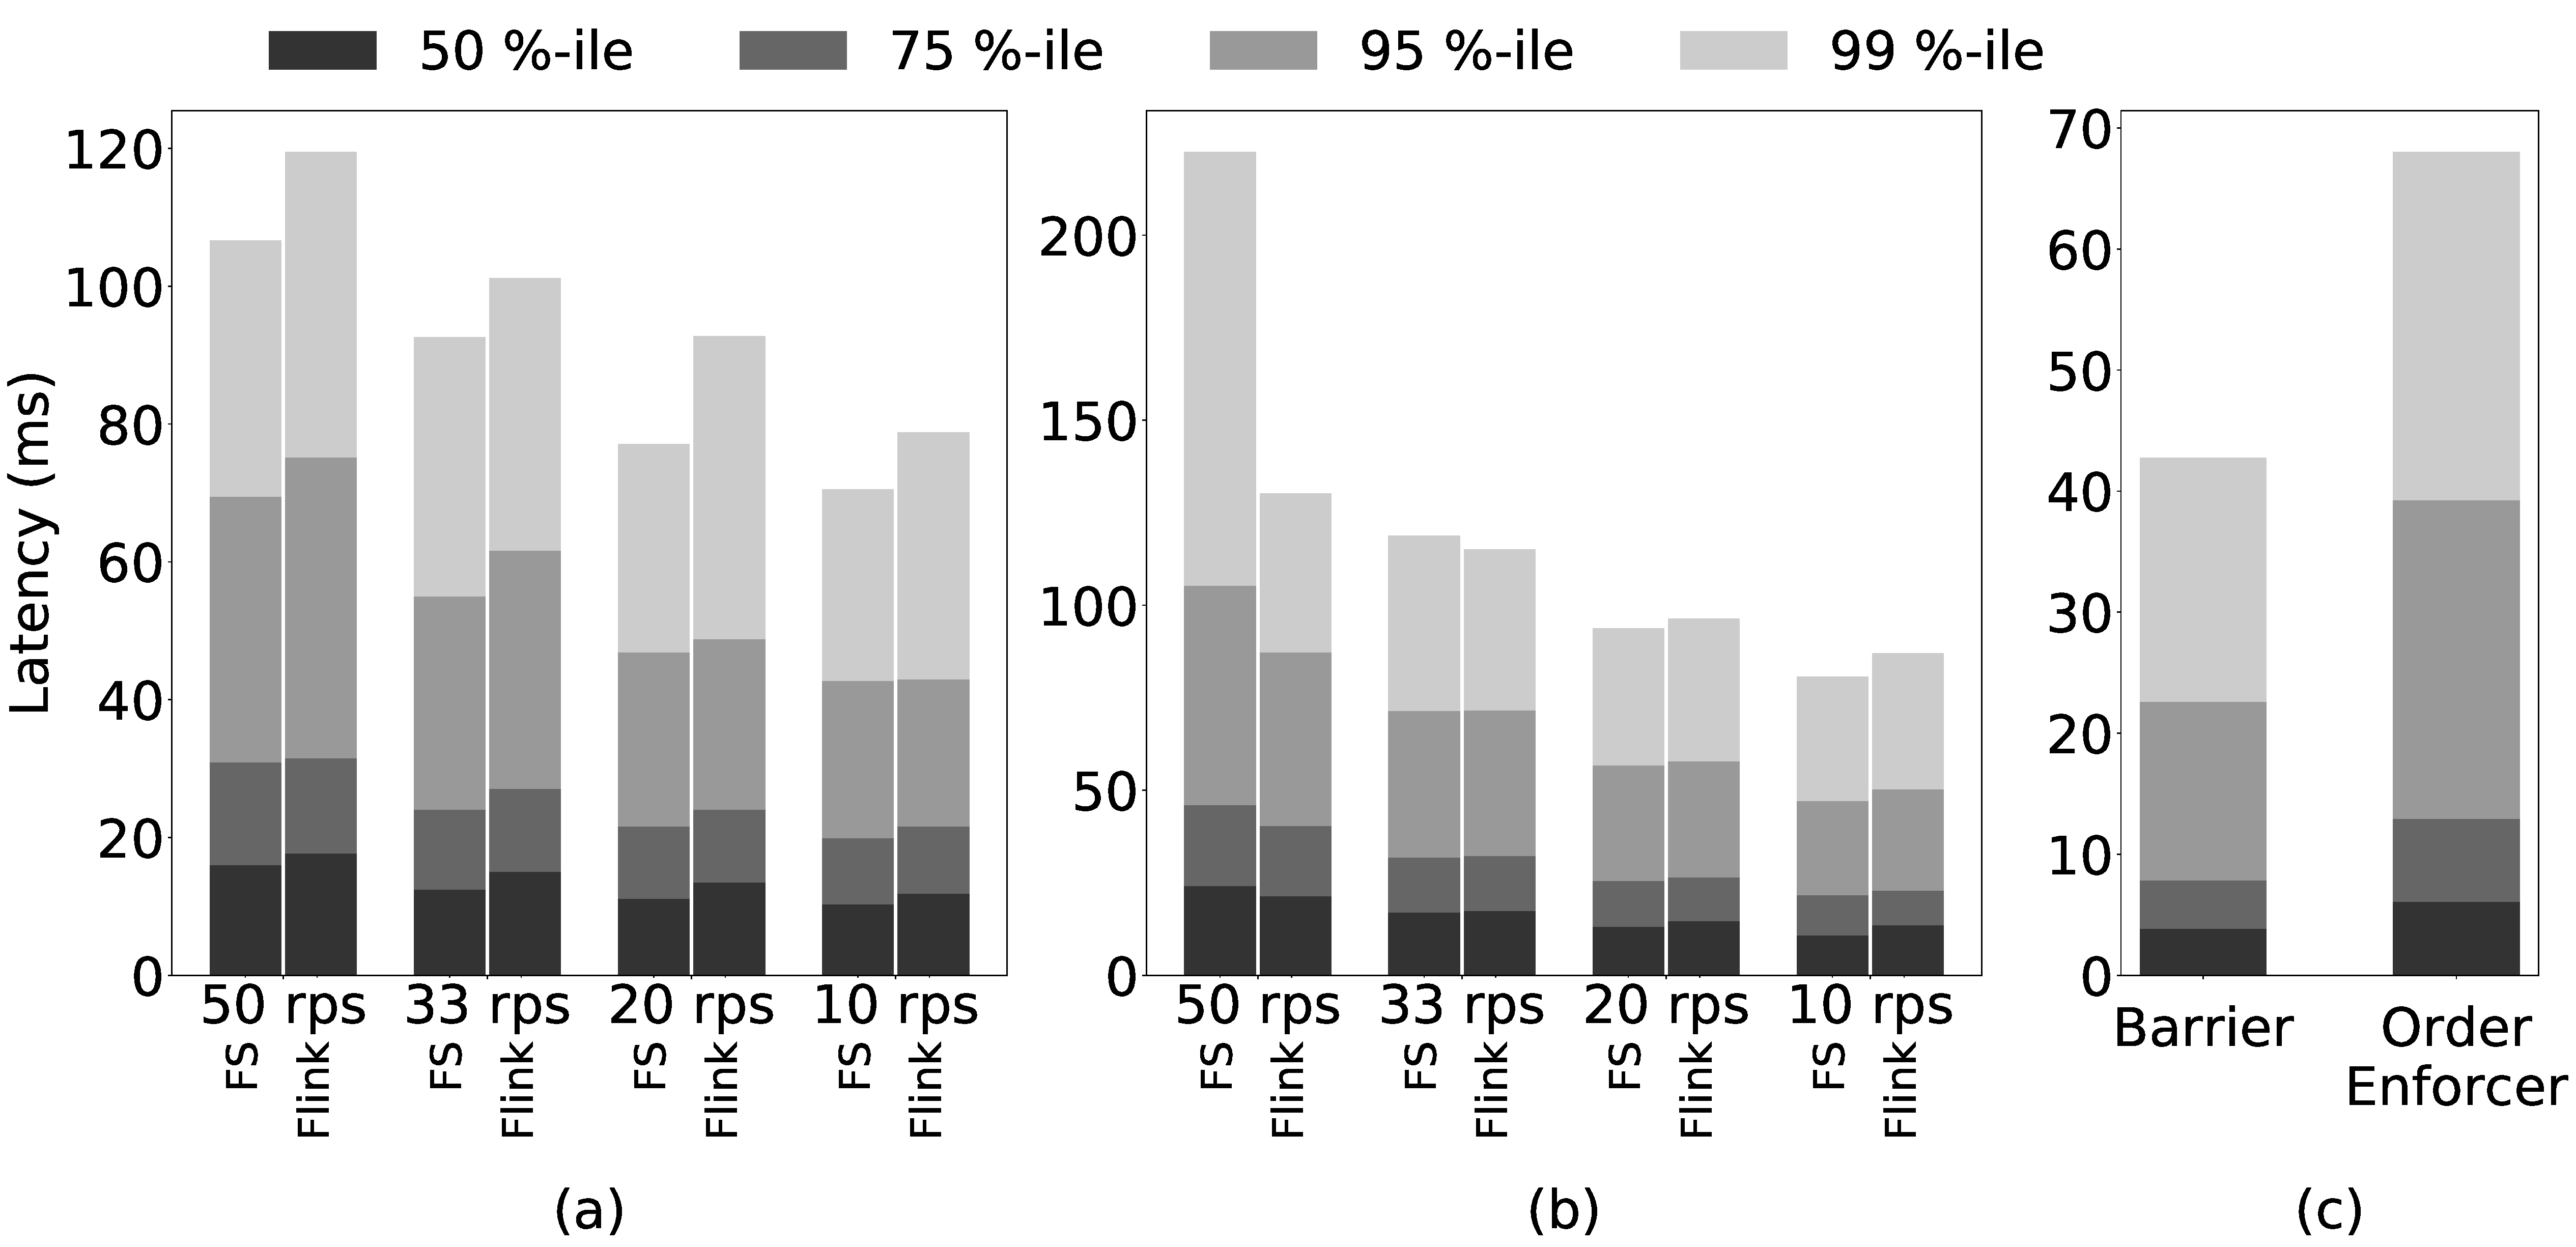
\includegraphics[width=0.25\textwidth]{pics/buffer-vs-barrier}
  \caption{Comparison between waiting time in Flink's buffer and FlameStream's barrier}
  \label {buffer-vs-barrier}
\end{figure}


\section {Related work}
%%%% fs-run-time-related  Related Work

\label {fs-related-section}

{\bf Data flow:}
One specific detail of our computational model is cyclic data flow graph support. Naiad~\cite{Murray:2013:NTD:2517349.2522738} by Microsoft Research provides an implementation of this idea. Nevertheless, Naiad applies cycles only for iterative computations and allows for each operation to have its own state. 

Another similar concept of Naiad is the usage of logical timestamps to monitor progress. However, to propagate the latest timestamp the pessimistic approach of notifications broadcasting is defined. Therefore, with the assumption of infrequent out-of-order items, our optimistic behavior is more relevant.

In our model, map and group operations are used as core processing primitives. Google Dataflow~\cite{Akidau:2015:DMP:2824032.2824076} provides the same idea. The primary distinction is that Google Dataflow model does not assume any kind of operation state. Additionally, this model provides different window types for grouping. FlameStream grouping is aligned with fixed-sized sliding window, but it is possible to implement other kind of windows by using cycle and grouping with window-affiliation hash.

{\bf State:}
The common approach to state management is to give a user the ability to handle a state of almost any supported operations. Such behavior is implemented, for isntance, in Apache Flink~\cite{carbone2015apache}, Storm~\cite{apache:storm}, Samza~\cite{Noghabi:2017:SSS:3137765.3137770}, Naiad~\cite{Murray:2013:NTD:2517349.2522738}.
To the best of our knowledge, FlameStream is the only open-source stream processing system that:
\begin{itemize}
    \item Stateless in terms of business-logic
    \item Supports any MapReduce transformations 
\end{itemize}

{\bf Tracking mechanisms within stream:}
One important task that FlameStream faces is handling of the minimal global time. In Apache Storm~\cite{apache:storm} acker is used to eliminate item traces. Unlike Strorm, we use acker to track the least global time of in-flight items and to detect package losses.


\section {Conclusion and future work}
%%% fs-run-time-conclu   Conclusions

\label {fs-conclusion-tection}

Some  of us are coders, but not writers.  Hopefully, almost everyone wil prove  the previos sentence is wrong.







\bibliographystyle{ACM-Reference-Format}
\bibliography{../../bibliography/flame-stream}
\end {document}


\endinput
you can put whatever here
